\chapter[Cryo-ET and STA]{Cryo-electron tomography and subtomogram averaging}

Tomographic reconstruction is not a recent invention: the first appearance goes back more than a century~\cite{jDeterminationFunctionsTheir1917}; its successful application to cryo-EM, however, is only a recent development closely linked to the resolution revolution, which allowed to finally overcome the biggest overarching limitation of cryo-ET --- poor signal-to-noise ratio --- enough to reach sub-nanometer resolutions~\cite{lucicCryoelectronTomographyChallenge2013,turkPromiseChallengesCryoelectron2020}.

At its core, cryo-ET is just cryo-EM with extra steps; they share much of the theory, hardware and software.
The key difference is that, where single particle cryo-EM uses projections from different \textit{copies} of the same object to reconstruct a 3D map, cryo-ET images the same location from multiple orientations in order to reconstruct a 3D map from multiple projections of the \textit{same} object.
This section describes the theory of cryo-ET, how it deviates from SPA, and the current state of the art with its limitations and upcoming developments.

\section{Sample preparation}
As with SPA, vitrification remains the key step of sample preparation for cryo-ET.
Due to the intrinsically worse SNR due to the lower electron dose used during data collection (\fullref{et_data_collection}), cryo-ET sample preparation requires extra care to reduce any possible source of additional noise.

One such source is the thickness of the sample; unfortunately, this is often antithetical to samples such as entire cells or organelles, where cryo-ET \textit{in situ} benefits really shine.
Initially, this problem was tackled by either prepararing simpler model systems \textit{in vitro} --- moving partly away from the native state --- or by cutting thin slices from a thicker sample via cryo-ultramicrotomy~\cite{peaseElectronMicroscopyUltramicrotomy1981}.
In recent years, focused ion beam (FIB) milling, a technique already well established in material sciences, has found widespread use in cryo-ET sample preparation, allowing to slice thin lamellae from a vitrified sample without incurring in the shear and surface deformations of cryo-ultramicrotomy~\cite{markoFocusedionbeamThinningFrozenhydrated2007}.

\subsection{FIB milling}
FIB milling typically makes use of a Gallium ion beam --- or, more recently, Xenon plasma --- to ablate a sample
thick samples can be thinned to below \qty{150}{\nano\meter}.
Preparing lamellae via FIB milling is becoming standard procedure in cryo-ET, but is still far from being consistently reproducible and automatable.

\begin{figure}[ht]
    \centering
    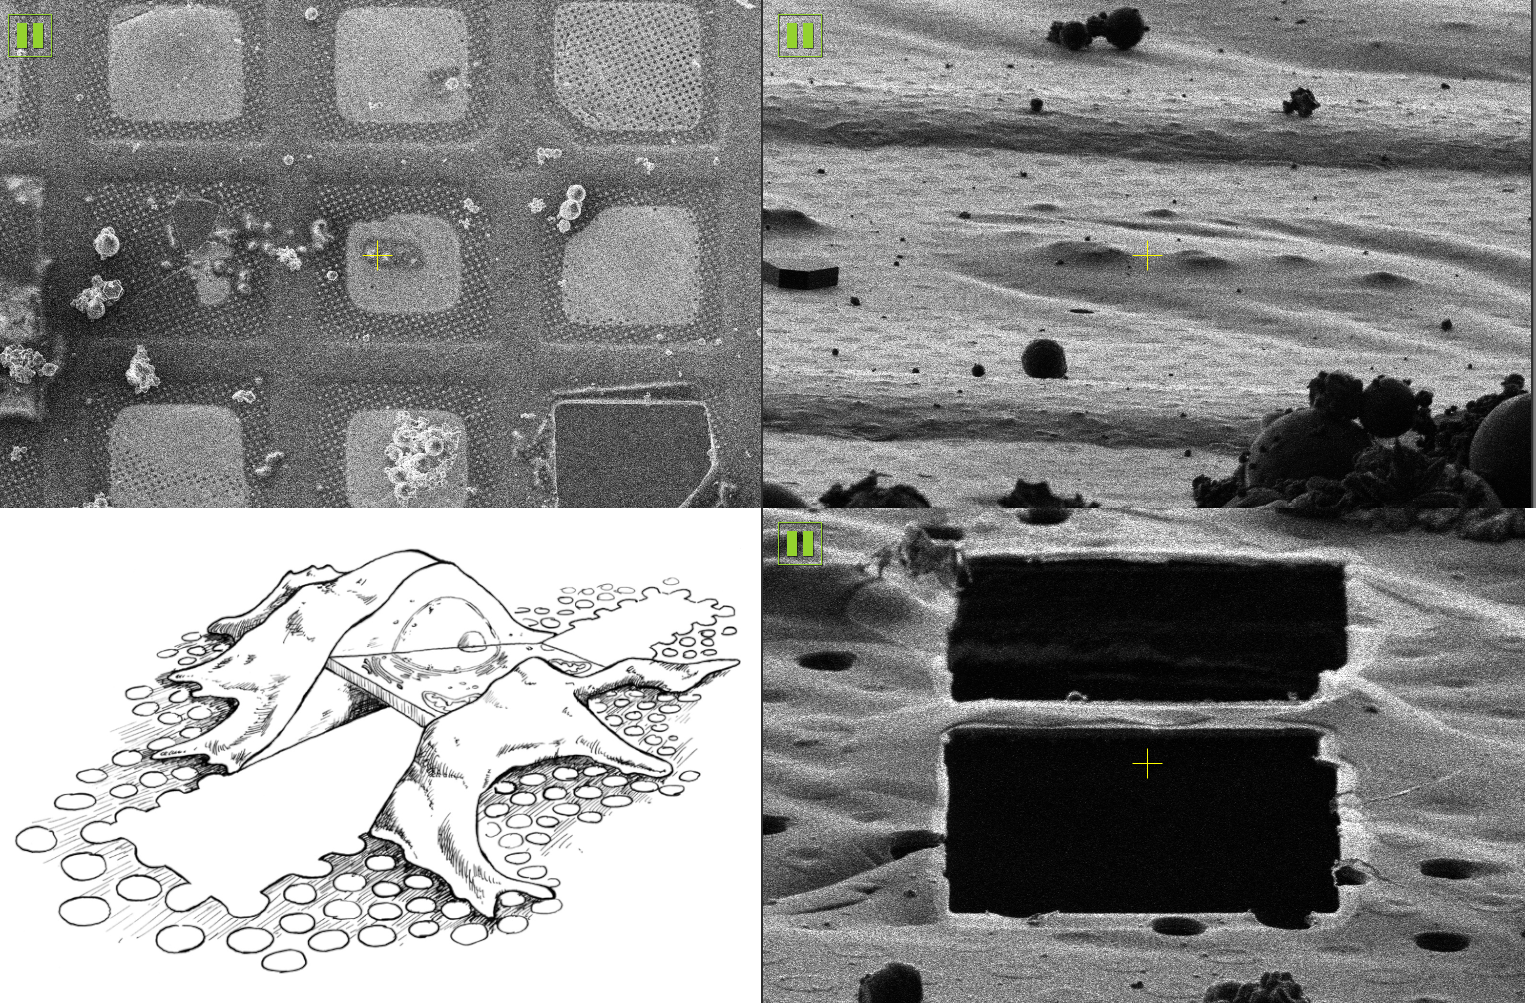
\includegraphics[width=\textwidth]{introduction/fib.png}
    \caption[FIB milling]{Microscope snapshots from FIB milling procedure on \textit{Deinococcus radiodurans}. A cluster of cells, visible as a bump on the SEM, is selected from the grid (top left). From a shallow angle of around \ang{15} from the grid (top right) the FIB is used to ablate material above and below the area of interest. This leaves a thin lamellae suitable for cryo-ET (bottom). Milled cell drawing (bottom left) taken from ~\citet{villaOpeningWindowsCell2013}.}
    \label{fig:et_fib_milling}
\end{figure}

TODO: CLEM perspectives?

\subsection{Fiducials}\label{fiducials}
During data collection, despite vitrification, samples undergo different kinds of deformations.
Moreover, due to the intrinsic imprecision of controlling the hardware of the microscope, there will always be some shift and angle mismatch between different tilts during a tilt series collection (\fullref{et_data_collection}).

To help with correcting these errors, it is often useful to add to the same some fiducials: small high-contrast, round objects (typically gold beads) that can later be used to estimate sample shift, rotation, and deformations (\fullref{et_tilt_series_alignment}).

\section{Data collection}\label{et_data_collection}
In order to acquire a sequence of images at different tilts (termed \textbf{tilt series}) for tomographic reconstruction, the same area of the sample needs to be imaged at a range of different angles.
This requires longer and more sophisticated routines compared to SPA, since for each tilt angle the sample stage must be moved, the eucentric height reestablished, the lens refocused.

Due to the multiple exposures, in order to preserve the specimen from radiation damage the electron duse must be fractionated to much lower than typical in SPA, but still high enough to capture enough signal to allow motion correction~\cite{mcewenRelevanceDosefractionationTomography1995}.

Each subsequent exposure further damages the sample, which degrades the high resolution information first.
This, in combination with the fact that in cryo-ET the electron beam has to traverse a thicker sample at high tilts --- leading to worse SNR --- created the need for optimized collection schemes.
The most commonly used nowadays is the Hagen (or dose-symmetric)  scheme~\cite{hagenImplementationCryoelectronTomography2017}: it collects the first image at \ang{0} tilt, and then alternates between negative and positive tilts until it reaches the maximum tilt.
This minimizes the radiation damage when SNR is best, allowing to capture high resolution information at its prime, before it is degraded.

Due to the geometry of the sample and its support within the microscope, there is a limit to how high an angle can be reached when tilting the sample.
This angle is typically around \ang{60}-\ang{70}, beyond which either the sample grid comes into view, or the sample becomes too thick for imaging at such low doses.
This will result in a \textbf{missing wedge} of information during tomographic reconstruction (\fullref{et_tomo_reconstruction}).

Conventional wisdom sets the interval between subsequent tilts at around \ang{3} to ensure enough fourier space filling while limiting radiation damage, though depending on the application --- especially where certain spatial frequencies are considered important or over-represented in the sample --- it might be worth considering smaller, wider, or non-linear increments~\cite{copeCryoElectronTomographyStructural2011}.

\section{Preprocessing}
Cryo-ET data undergoes similar preprocessing steps as SPA data (\fullref{em_preprocessing}), albeit with less precision due to the low electron dose.

While at this point single particle data is ready for particle picking and other downstream work, cryo-ET data must still undergo tomographic reconstruction in order to obtain the 3D volumetric reconstruction of the sample.

To do so, tilt series alignment parameters must first be estimated in order to correct for equipment imprecision and sample deformations, and then used the 3D volume reconstruction.

\subsection{Tilt series alignment}\label{et_tilt_series_alignment}
The most basic alignment procedures require at least full-frame aligment; similar to motion correction, tilt images are rotated and shifted in order to maximize their CC score.
Where fiducials are present (\fullref{fiducials}), these can be treated as static points within the sample and used instead as anchors to mathematically estimate the geometric transformation between different tilts~\cite{nicastroMolecularArchitectureAxonemes2006,heumannClusteringVarianceMaps2011,castano-diezDynamoCatalogueGeometrical2017}.

In state of the art software, alignment procedures (with or without fiducials) can also account for spatio-temporal deformations of the sample, either already during tilt series alignment~\cite{zhengAreTomoIntegratedSoftware2022}, or later during refinement~\cite{tegunovMultiparticleCryoEMRefinement2021,burtImageProcessingPipeline2024,galaz-montoyaSingleParticleTomography2015,chenCompleteDataProcessing2019} (\fullref{et_refinement}).

\subsection{Tomogram Reconstruction}\label{et_tomo_reconstruction}
Similarly to how 3D reconstructions are obtained from 2D particles in SPA based on the central slice theorem (\fullref{em_reconstruction}), the aligned tilt series can be used to reconstruct the full tomogram.
Depending on the software suite and workflow, full tomogram reconstructions may be used only for template matching (\fullref{et_particle_picking}) and segmentation purposes, or also to extract subtomograms at small pixel sizes for subtromogram averaging (\fullref{et_sta}).

Differently from SPA, cryo-ET has the advantage of knowing the 3D positioning of features in the tomogram.
This allows to bring defocus estimation and CTF correction to the next level: not only is CTF locally estimated depending on the in-plane position of features, but also accounting for the defocus difference between the top and bottom of the sample.
While this idea was around for a long time, only in recent years tools were developed that can run in reasonable time and significantly improve the final resolution~\cite{turonovaEfficient3DCTFCorrection2017,tegunovRealtimeCryoelectronMicroscopy2019}. 
Depending on the software, 3D-CTF might be estimated and corrected at different levels (tilt image, full tomogram or subtomogram), and may be able to be refined during refinement (\fullref{et_refinement}).

Due to the limited range of tilt angles collected in typical cryo-ET workflows, not all views of the sample are represented; when reconstructing the 3D FT of the sample, this is clearly visible in in fourier space as a wedge of missing information (\autoref{fig:et_missing_wedge}).
The missing wedge introduces several problems in downstream processing: it blurs the tomogram in the Z direction, it biases subtomogram alignment, and it leads to anisotropic resolution for objects with preferential orientation.

If fiducials (or other high-contrast objects of no real interest) are present in the sample, it is often useful to mask them during reconstruction, in order to avoid the high-contrast artifactual streaks caused by the missing wedge, which can impair the interpretability of the tomogram~\cite{tegunovRealtimeCryoelectronMicroscopy2019,burtTeamtomoFidder2024}.

\begin{figure}[ht]
    \centering
    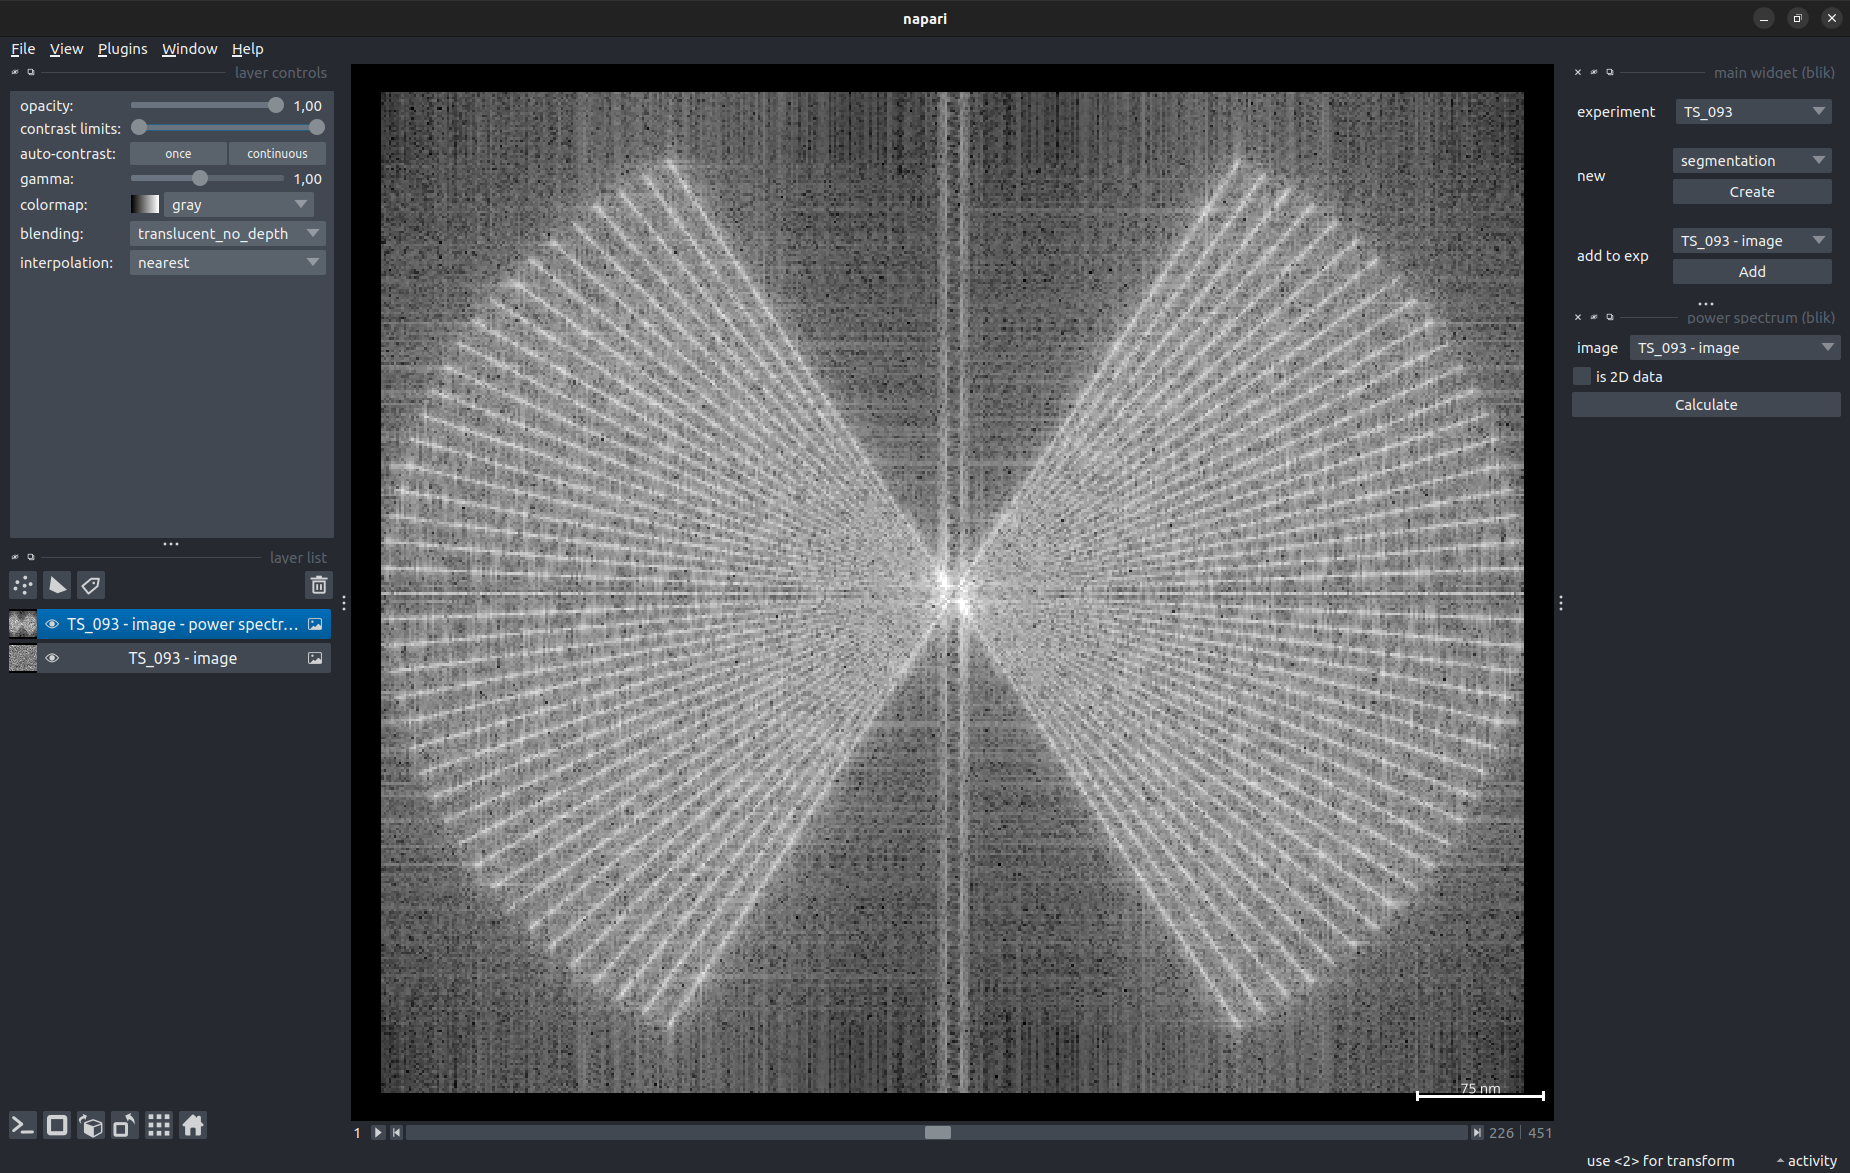
\includegraphics[width=\textwidth]{introduction/missing_wedge.png}
    \caption[Missing wedge]{2D slice through the 3D FT of a tomogram, perpendicular to the tilt axis. The 2D FT of images of the tiltseries are visible as lines at regular angular spacing; at the top and bottom they are not present, creating the missing wedge.}
    \label{fig:et_missing_wedge}
\end{figure}

TODO: missing wedge correction (isonet)

\section{Annotation and segmentation}\label{et_annotation_segmentation}
Thanks to the \textit{in situ} and quasi-native nature of tomography data, it is often useful to annotate or segment tomograms in order to get a better view of the morphology of the sample, or to find areas and particles of interest more easily.

One of the most common approaches is to do semantic segmentation (aka labeling), where individual voxels are assigned a type --- "membrane", "ribosome", and so on, though usually in the form of a integer --- either by manually painting over the sample, or automatically via image processing algorithms or ML tools.
Labeling helps with visualisation by boiling down the sample to its most fundamental components, while also serving as a powerful tool for quantitative and morphological analysis of complex mesoscale objects.
To this end, segmentations are often used as starting point for other kinds of annotations, such as abstracting membranes or filaments to mathematical objects like splines and skeletons (CITE skan?) in order to calculate properties such as membrane curvature, filament branch length, and so on.

In some projects, morphology is all that matters, with no need to reach high resolution; in such cases, the cryo-ET pipeline can stop after annotation.
Where high resolution molecular structures are the goal, segmentations and other annotations may also be used as a starting point for particle picking.

\section{Particle picking}\label{et_particle_picking}
Picking particles in tomograms is not so different from picking particles from 2D micrographs, other than having an extra dimension.
Manual picking and template matching are still the preferred methods, though more and more software is developed for ML-based or hybrid methods (CITE cryolo, ...).

TODO: manual picking harder cause 3rd dimension (filaments...), crowding, missing wedge

As with most things in cryo-ET, low SNR is the main obstacle to overcome; this is why some picking tools --- such as the one developed during this thesis (\fullref{blik}) --- attempt to use as much prior knowledge about the system as possible in order to limit the degrees of freedom when searching for particles~\cite{castano-diezDynamoCatalogueGeometrical2017,wagnerEvolutionSPHIREcrYOLOParticle2020,gaifasBlikExtensible3D2024}.

Whenever possible, segmentation or other kinds of annotation can be used as baseline for particle picking: either by masking areas of interest --- such as picking only inside a certain cellular structure --- or by seeding particle picks based on the annotation geometry --- such as distributing particles on the surface of a membrane.
Such information may also be used to initialize the particle orientation to something self-consistent (e.g: all perpendicular to the membrane); this can affect drastically the initial model generation and subsequent refinement, where 3D rotational search may otherwise not overcome the SNR.

\section{Subtomogram averaging}\label{et_sta}
In cryo-ET, the equivalent to SPA's 2D classificatin and 3D refinement is subtomogram averaging (STA).
The idea at the core is the same: by combining the data from many subvolumes extracted from the tomogram (subtomograms) which contain copies of the same object, the SNR can be drastically improved.
The basic procedure is also very similiar to SPA, only in 3D: subtomograms are extracted from the full reconstructed tomogram based on the positions of the particle picks; then, rounds of cross-correlation and refinement (and/or classification) improve the model until convergence (\fullref{em_classification}).

In recent years, however, the field is moving away from this naive approach where "rigid" subtomograms are extracted from a full 3D reconstruction, in favor of directly reconstructing subtomograms from the 2D data, using what is sometimes called \textbf{per-particle tilt series}~\cite{zivanovBayesianApproachSingleparticle2022,tegunovRealtimeCryoelectronMicroscopy2019,chenCompleteDataProcessing2019}.
This opens up many avenues for optimization --- such as 3D-CTF correction (\fullref{et_tomo_reconstruction})~\cite{turonovaEfficient3DCTFCorrection2017}, multi-particle refinement~\cite{tegunovMultiparticleCryoEMRefinement2021} or bayesian polishing~\cite{zivanovBayesianApproachSingleparticle2022} --- by not allowing the subtomogram reconstruction parameters to be tweaked after the first reconstruction (\fullref{em_refinement}).

A significant obstacle during alignment is caused by the missing wedge; it is such a prominent feature that during cross-correlation, it would normally overpower everything else in the subtomograms.
Because of this, subtomograms would end up being rotationally aligned based on how they are rotated relative to the missing wedge, instead of their relative rotation to each other.
For this reason, missing wedge compensation is a crucial step for the success of STA procedures~\cite{galaz-montoyaAlignmentAlgorithmsPerparticle2016} (CITE more).

\section{Refinement}\label{et_refinement}

TODO: not sure if there's anything else to say here, maybe no need.

\section{Pros and Cons}

Cryo-ET has seen a rapid development in recent years, bringing it to the forefront of structual biology techinques.

By providing a high resolution, \textit{in situ} view of biological systems, it brings insights that other \textit{ex situ} techniques like X-ray crystallography and SPA cannot provide.
At the same time, thanks to STA, cryo-ET is able to bridge the gap with single particle analysis, reaching in some cases sub-nanometer resolution for single particle structures, while maintaining the ability to contextualize such structures within the complex biological system they belong to.

A distinctive strength of cryo-ET is the ability to explore mesoscale systems or superstructures --- such as folded 2D lattices and filaments --- without trivializing them for bottom up, \textit{in vitro} reconstitution, and instead observing their structural arrangement as it behaves \textit{in situ}.

Many of cryo-ET's limitations are utlimately ascribable to the low SNR; some of them can be overcome with hardware improvements (better sample preparation, detectors and phase plates), and others with software advances (chromatic aberration correction, better alignment and refinement procedures).
In recent years, several groups are working on developing new hardware and software for cryo-EM and cryo-ET, steadily improving the attainable resolution (\autoref{fig:et_smallest_particle})~\cite{russoCryomicroscopySituWhat2022}.

\begin{figure}[ht]
    \centering
    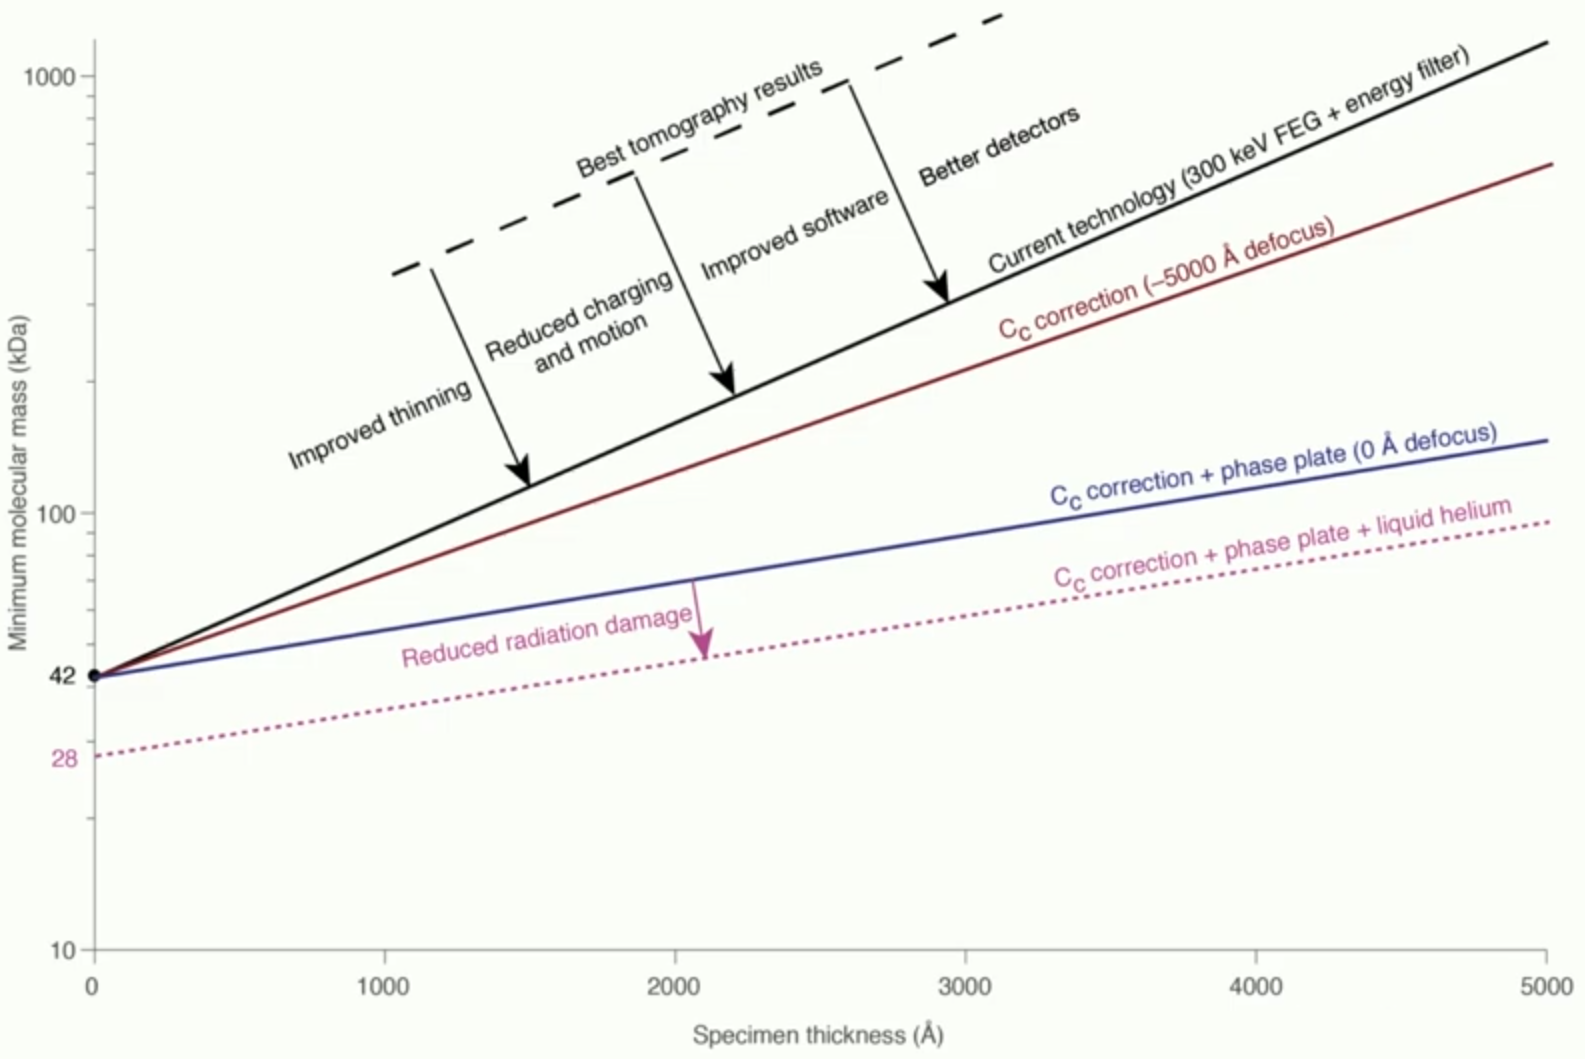
\includegraphics[width=\textwidth]{introduction/smallest_particle_plot_russo.png}
    \caption[Particle size limit in cryo-ET]{Theoretical lower limit of particle size that can be resolved via cryo-ET, depending on the sample size. Currently, even the best tomography results are far from the theoretical limits due to lack of optimization in sample preparation and hardware. The current theoretical limits can yet be improved by implementing some additional methods. Figure taken from \citet{russoElectronCryomicroscopeHardware2023}.}
    \label{fig:et_smallest_particle}
    % TODO: find better version? Ask chris?
\end{figure}

Another common hurdle, especially for researchers new to cryo-ET, is presented by the messy and fragmented software ecosystem.

\begin{outline}
\1 \tick base concepts and differences from SPA from thechnical standpoint
    \2 \tick cryoem, but different data acquisition and thus data processing
    \2 \tick exposure damage and dose issues
    \2 \tick sample prep (thinnes especially important because SNR)
    \2 \tick tilt-series alignment (fiducials), deformation, other aberrations, how they are tackled
    \2 \tick 3D CTF
    \2 \tick missing wedge, issues it introduces
    \2 \tick feature deletion (e.g: fiducials)
    \2 \tick segmentation/morphology
    \2 \tick STA (picking, averaging, classification, ...) for non-unique objects (template matching, geometric and template free, machin learning)
\1 \tick some references/reviews (cool stuff you can do)
    \2 \tick \cite{turkPromiseChallengesCryoelectron2020,lucicCryoelectronTomographyChallenge2013}
\1 what it provides compared to SPA
    \2 \tick more native state and context preservation
    \2 \tick single-particle insights
    \2 \tick mesoscale and superstructural information
\1 limitations (both in terms of technique, and in terms of current state of development)
    \2 \tick (some mentioned before, maybe need to connect these two parts a bit better)
    \2 \tick need for custom workflow cause the goal and problems are usually unique
    \2 \tick issues caused by the missing wedge (alignement, reconstruction, interpretability)
    \2 \tick SNR, denoising
    \2 visualisation/interaction
    \2 object identification (crowding)
\1 related techinques to overcome some limitations
    \2 \tick FIB, what it enables and how it works
    \2 CLEM
\end{outline}
